\documentclass[12pt,pdftex,a4paper]{scrartcl}
\usepackage{scrlayer-scrpage}
\usepackage[utf8]{inputenc}
\usepackage[english]{babel}
\usepackage{listings,graphicx,multirow,xcolor}
\usepackage[hyphens]{url}
\usepackage[bf,sf]{caption}
\usepackage{subcaption}
\DeclareCaptionLabelFormat{plain}{Fig. #2}
\captionsetup[figure]{labelformat=plain,labelsep=quad}

\begin{document}
\title{Automatic role labeling}
	\subtitle{Emotion analysis -- assignment 4}
	\author{Carlotta Quensel\\Felix Bühler\\ Maximilian Wegge}
	\maketitle


\section{Introduction}
As the task of sequence labelling is more advanced than whole-text emotion classification, we expect there to be more difficulties in automatic labelling as well as bigger differences between na\"{i}ve and complex algorithms.

Thus, we decided to do automatic role labeling to confirm these expectations. The sequences for emotion experiencer, target or stimulus are mostly semantically determined and do not directly map onto syntactic structures, but the difference in syntactic structure between different training data might still hold an effect on the results. In this assignment, we look to answer if and how a naive and complex sequence labelling approach differ, as well as compare the influence of different training data on the results. With these objectives as our research questions, we now are able to decide on our method and data.

\section{Method}
Both methods are trained on the same data, so that we can compare the intersection between data and algorithm influences. Therefore, our first step in implementing a role labelling algorithm is to decide on the different data.
\subsection{Training data}
To keep the task mamageable, we only label one role, which is target. The semantic role of emotion target might in a na\"{i}ve understanding correspond to the syntactic role of object (e.g. \textit{I am angry at \textbf{you}.}). This is of course not correct in many instances but still opens an interesting distinction between corpora. As the Reman corpus consists of literary texts, GoodNewsEveryone of news headlines and Electoral tweets of tweets, these three corpora have very different syntactic styles, the news being abbreviated and the literature containing more complex syntactic contructs. While the distribution of our selected role is not ideal between the corpora (Reman only contains around 700 target instances), going forward, these are the three corpora used for training and evaluating both algorithms.

\subsection{Na\"{i}ve approach -- Hidden Markov model}
Sequence labelling in general and the role labelling of emotion target specifically is dependent on the word order, sentence semantic and therefore also syntactical information. While both approaches only consider the tokens as labelling information, while the complex method learns to hopefully detect underlying structures in the token order, the simple method only considers the order of labels. As a basic sequence labelling method, we chose to train a Hidden Markov model and then determine the best label sequence using a viterbi algorithm (the code can be found at the end of this documentation). The model is trained with the token-label pair frequencies relative to the token frequency as emission probabilities and the label bigram frequencies relative to the second token as transition probabilities. An estimated best label sequence therefore combines the most probable label sequence with the highest possibilities of labels for each individual token. The viterbi algorithm is then used to compute this most probable label sequence for a given token sequence. 

While Hidden Markov models have many applications in natural language processing, as a sequence labelling algorithm, it is most frequently used for POS-tagging. In contrast to POS-tagging, a HMM in our case has a deficit, as the tokens are not connected to the tags as strongly. Even though a token can change its syntactical category according to its place in the sentence, there are generally only a few possible labels it can take on. For emotion role labelling on the other hand, a sequence like \textit{my mother} can be the emotion target as well as the experiencer or even the stimulus. The classification mostly depends on semantic information which might be transported through syntactic structure, which our approach does not take into account, as the tokens themselves are only counted as unigrams. Thus, we use a more complex learning approach to combat the problem of missing context. 

\subsection{Complex approach -- Transformer}\label{sec:trans}
For the complex approach, we chose RoBERTa. This deep learning method is an extension of the BERT transformer, which means it is pre-trained on external data. We used 'RoBERTa' to convert the tokenized sentences into an input matrix. This way we can use the whole sequence as context for each individual token. We set a maximum word amount to 100 words, because most of the sequences in our corpora are shorter. The first layer is the pre-trained RoBERTa model\footnote{RoBERTa distribution: \url{https://huggingface.co/transformers/model_doc/roberta.html}}, which was not re-trained, as it has 124 million parameters and therefore superseeds our spacial and temporal constraints. The output is then fed into a bidirectional LSTM with 64 units. Its output is in turn fed into another bidirectional LSTM of the same make-up. Then we used a Dense-Layer to combine all the features. Thus, the model has the architecture shown in figure \ref{arch}. Adding a residual connection between the first LSTM and the Dense-Layer improved our accuracy. These layers are used in a Time-Distributed-Layer to produce a prediction for each token. For learning we also added 'ReduceLROnPlateau' to reduce the learning-rate for internal metrics when learning stagnates.

\begin{figure}
\centering 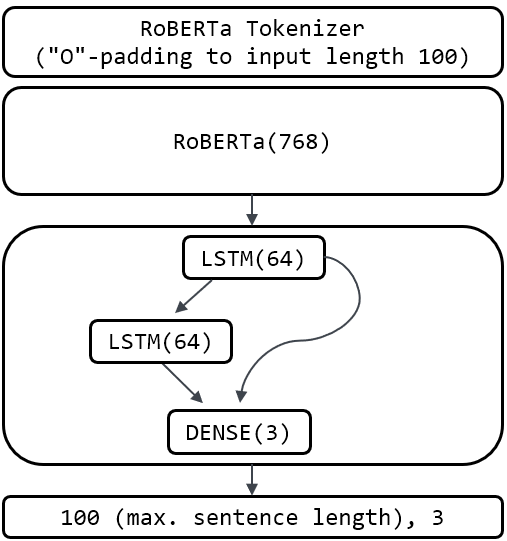
\includegraphics[width=.45\textwidth]{roberta-arch} 

\caption{Model architecture of the RoBERTa with an input layer size of 100 and an output of 3 ('O', 'B' and 'I') for each of the 100 input dimensions.}\label{arch}
\end{figure}

A difficulty with this approach is the sentence length. Since all inputs have the same length, we pad shorter sequences with additional 'O's, thus the model predicts 'outside' at a disproportionate frequency considering the real label counts in the corpora. Reducing the amount of words could improve the predictions, but important information could be cut off (only a problem with the Reman data, as the sentences are very complex and long). Using RoBERTa also influenced the time requirements of our training, e.g. training on "Good News Everyone" took about 3 hours.

\section{Evaluation}
In opposition to token-wise evaluation, evaluation of sequences can be ambiguous. In this approach to evaluation, we count intersections between the gold and predicted sequence as correct labels (True Positives) without differentiating between 'B' and 'I'. When a gold label sequence spans more than one predicted sequence, we only count one of these multiples and ignore the rest. 

\begin{figure}[h!]
\centering 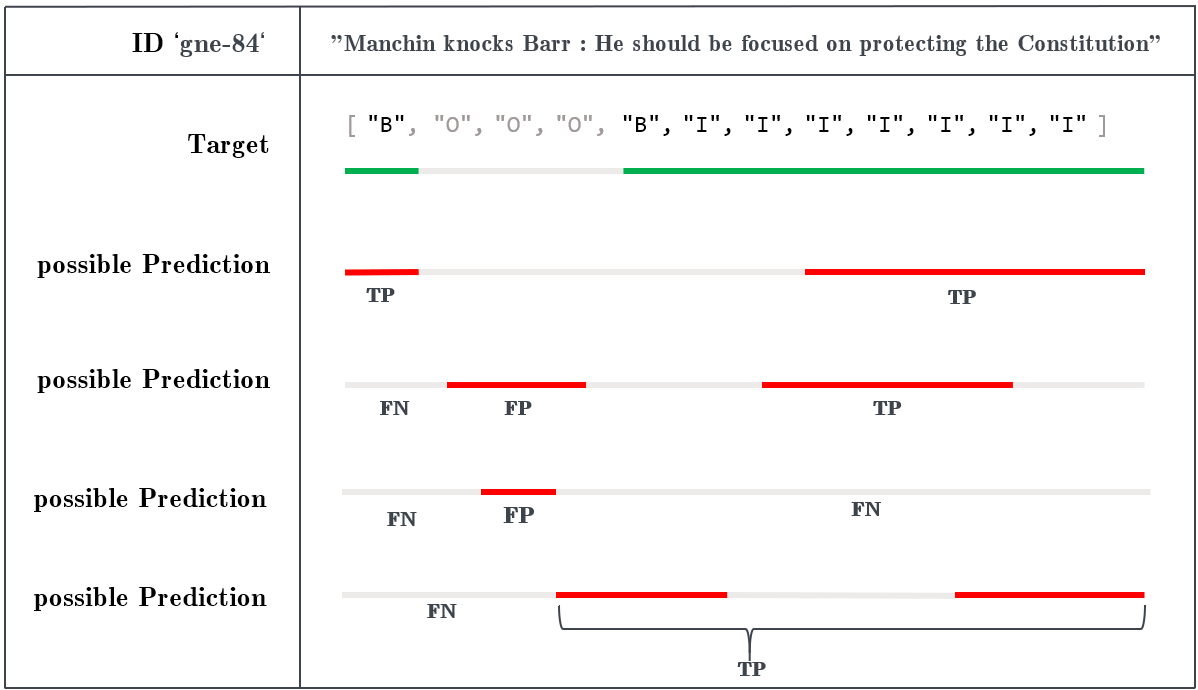
\includegraphics[width =.8\textwidth]{eval}
\caption{Example predictions for the target sequence and their categorization as correct and incorrect.}\label{fig:eval}
\end{figure}

Analogously, incorrect predictions are defined as empty intersections: False Negatives are counted if the model does not predict a target sequence, False Positives if it predicts a non-target sequence. In this evaluation, we do not count True Negatives (correctly predicted non-target sequence), as they do not contribute to precision, recall and f-score for the target sequence and would add further ambiguity to the evaluation process. Figure \ref{fig:eval} illustrates this approach with some examples (note that the predictions are created manually to best show different cases and do not represent the actual output of our models). In applying this method, we yield the following results for both models and all three training corpora respectively.

% Matrix TP, FN, FP für viterbi x gne
    \begin{figure}[h!]
        \centering
        \begin{subfigure}{0.3\textwidth}
        \begin{tabular}{c c | c c c}
            & & \multicolumn{3}{c}{\textbf{Gold}} \\
            & & \textbf{In} & & \textbf{Out} \\ \hline
            & & & & \\
            \multirow{-1.5}{*}{\rotatebox{90}{\parbox{2cm}{\centering \textbf{Predicted}}}}
            & \textbf{In} & 2132 & & 5788 \\
            & & & & \\
            & \textbf{Out} & 1559 & & n.a. \\
            \smallskip \\ \hline \hline
            \multicolumn{3}{l}{\textbf{precision:}} & \multicolumn{2}{r}{0.269}\\
            \multicolumn{3}{l}{\textbf{recall:}} & \multicolumn{2}{r}{0.578}\\
            \multicolumn{3}{l}{\textbf{f-score:}} & \multicolumn{2}{r}{0.370}\\
        \end{tabular}
        \caption{trained on GNE}\label{eva-vit-gne}
        \end{subfigure}\hfill
        \begin{subfigure}{0.3\textwidth}
        \begin{tabular}{c c | c c c}
            & & \multicolumn{3}{c}{\textbf{Gold}} \\
            & & \textbf{In} & & \textbf{Out} \\ \hline
            & & & & \\
            \multirow{-1.5}{*}{\rotatebox{90}{\parbox{2cm}{\centering \textbf{Predicted}}}}
            & \textbf{In} & 4365 & & 11739 \\
            & & & & \\
            & \textbf{Out} & 1026 & & n.a. \\
            \smallskip \\ \hline \hline
            \multicolumn{3}{l}{\textbf{precision:}} & \multicolumn{2}{r}{0.271}\\
            \multicolumn{3}{l}{\textbf{recall:}} & \multicolumn{2}{r}{0.810}\\
            \multicolumn{3}{l}{\textbf{f-score:}} & \multicolumn{2}{r}{0.406}\\
        \end{tabular}
        \caption{trained on Elec. Tweets}\label{eva-vit-et}
        \end{subfigure}\hfill
        \begin{subfigure}{0.3\textwidth}
        \begin{tabular}{c c | c c c}
            & & \multicolumn{3}{c}{\textbf{Gold}} \\
            & & \textbf{In} & & \textbf{Out} \\ \hline
            & & & & \\
            \multirow{-1.5}{*}{\rotatebox{90}{\parbox{2cm}{\centering \textbf{Predicted}}}}
            & \textbf{In} & 6335 & & 11087 \\
            & & & & \\
            & \textbf{Out} & 1099 & & n.a. \\
            \smallskip \\ \hline \hline
            \multicolumn{3}{l}{\textbf{precision:}} & \multicolumn{2}{r}{0.364}\\
            \multicolumn{3}{l}{\textbf{recall:}} & \multicolumn{2}{r}{0.852}\\
            \multicolumn{3}{l}{\textbf{f-score:}} & \multicolumn{2}{r}{0.510}\\
        \end{tabular}
        \caption{trained on Reman}\label{eva-vit-re}
        \end{subfigure}
        
        \caption{All three Hidden Markov models with viterbi predictions that are trained on one corpus, and evaluated on the other two.}\label{eva-vit}        
    \end{figure}


% Matrix TP, FN, FP für transformer x electweets
    \begin{figure}[h!]
        \centering
        \begin{subfigure}{0.3\textwidth}
        \begin{tabular}{c c | c c c}
            & & \multicolumn{3}{c}{\textbf{Gold}} \\
            & & \textbf{In} & & \textbf{Out} \\ \hline
            & & & & \\
            \multirow{-1.5}{*}{\rotatebox{90}{\parbox{2cm}{\centering \textbf{Predicted}}}}
            & \textbf{In} & x & & x \\
            & & & & \\
            & \textbf{Out} & x & & n.a. \\
            \smallskip \\ \hline \hline
            \multicolumn{3}{l}{\textbf{precision:}} & \multicolumn{2}{r}{0.x}\\
            \multicolumn{3}{l}{\textbf{recall:}} & \multicolumn{2}{r}{0.x}\\
            \multicolumn{3}{l}{\textbf{f-score:}} & \multicolumn{2}{r}{0.x}\\
        \end{tabular}
        \caption{trained on GNE}\label{eva-trans-gne}
        \end{subfigure}\hfill
        \begin{subfigure}{0.3\textwidth}
        \begin{tabular}{c c | c c c}
            & & \multicolumn{3}{c}{\textbf{Gold}} \\
            & & \textbf{In} & & \textbf{Out} \\ \hline
            & & & & \\
            \multirow{-1.5}{*}{\rotatebox{90}{\parbox{2cm}{\centering \textbf{Predicted}}}}
            & \textbf{In} & 15 & & 57 \\
            & & & & \\
            & \textbf{Out} & 4552 & & n.a. \\
            \smallskip \\ \hline \hline
            \multicolumn{3}{l}{\textbf{precision:}} & \multicolumn{2}{r}{0.208}\\
            \multicolumn{3}{l}{\textbf{recall:}} & \multicolumn{2}{r}{0.003}\\
            \multicolumn{3}{l}{\textbf{f-score:}} & \multicolumn{2}{r}{0.006}\\
        \end{tabular}
        \caption{trained on Elec. Tweets}\label{eva-trans-et}
        \end{subfigure}\hfill
        \begin{subfigure}{0.3\textwidth}
        \begin{tabular}{c c | c c c}
            & & \multicolumn{3}{c}{\textbf{Gold}} \\
            & & \textbf{In} & & \textbf{Out} \\ \hline
            & & & & \\
            \multirow{-1.5}{*}{\rotatebox{90}{\parbox{2cm}{\centering \textbf{Predicted}}}}
            & \textbf{In} & 112 & & 330 \\
            & & & & \\
            & \textbf{Out} & 7322 & & n.a. \\
            \smallskip \\ \hline \hline
            \multicolumn{3}{l}{\textbf{precision:}} & \multicolumn{2}{r}{0.253}\\
            \multicolumn{3}{l}{\textbf{recall:}} & \multicolumn{2}{r}{0.015}\\
            \multicolumn{3}{l}{\textbf{f-score:}} & \multicolumn{2}{r}{0.028}\\
        \end{tabular}
        \caption{trained on Reman}\label{eva-trans-re}
        \end{subfigure}
        \caption{Three RoBERTa models each trained on GNE, Electoral-Tweets,
        or Reman and evaluated on the other two corpora.}\label{tab:eval_trans}
    \end{figure}

\subsection{Comparison of models}
As shown in the figures \ref{eva-vit} and \ref{tab:eval_trans}, the na\"{i}ve approach of  our Hidden Markov model surprisingly produces significantly better results than the more complex RoBERTa. This can be partly explained by both methods' training requirements. The HMM bases the predicted sequence partially on the most likely tag transitions, which means that 'B' or 'I' is more often than not followed by another 'I', resulting in longer and more predicted sequences. The transformer on the other hand needs an input of constant length, as explained in section \ref{sec:trans}. By evaluating the models together with the above explained evaluation method, the HMM gets an advantage over the transformer.

However, the HMM predicts too many and too long sequences, as can be seen by the low precision in contrast to the relatively high recall. Due to our evaluation method, a model predicting the whole text as one sequence will lead to a precision and recall of 1, as whole sequences are always counted as correct if they intersect with the gold sequence, even if they also intersect large sequences of outside tokens. In opposition to the transformer, it is too greedy.

The transformer learns too many 'O's from the padded sequences and will therefore predict much less sequences and often predict no emotion target in the sentence at all. Thus, the recall is bad (between 0 and 1\% of target sequences are found) while the precision is worse but comparable to that of the HMM. 

The faults of both models are clearly visible when comparing results directly. The sentence below (ID: gne-1547) has a gold target sequence marked in bold which for human annotators would be fairly simple to annotate.


\begin{tabular}{cccccccccc}
\textit{These} & \textit{Artists} & \textit{Want} & \textit{to} & \textit{Blow} & \textit{Up} & \textit{the} & \textbf{\textit{Whole}} & \textbf{\textit{Financial}} & \textbf{\textit{System}}
\medskip\\
\multicolumn{10}{l}{\textbf{HMM:}}\\
B & I & I & I & I & I & I & I & I & I\\
\multicolumn{10}{l}{\textbf{RoBERTa:}}\\
O & O & O & O & O & O & O & O & O & O\\
\end{tabular}

When comparing the predictions of the Hidden Markov model and the transformer, both of which are trained on the same data from the Reman corpus, we see the opposition of the models' problems. While the HMM predicts the whole sentence to be a target, the RoBERTa model predicts no target sequence at all. For further evaluation, we can therefore conclude that both models struggle with a meaningful recall, either the score is not informative or too low.

As the precision for both models is quite low, we might consider that a token only approach is not the best method for this task of sequence labelling. Instead, the model could additionaly take POS-tags or even simple syntactical sequences (chunks) as input. The Hidden Markov model is an Ngram model and could thus be extended to consider token bigrams instead of unigrams in its emission probabilities.

\subsection{Comparison of training corpora}
For the simpler model, the training data that leads to the best results is the Reman corpus. This is somewhat surprising, as it includes the least amount of annotated emotion targets and is thus very sparse for training. On the other hand, as the texts in the corpus are sentences from literature, the original writer likely structured them deliberately, leaving less room for errors that result from bad grammar or colloquial language. Reman significantly improves the precision with regard to the other training corpora, as the biggest flaw of annotating too many or too long sequences is somewhat reduced with this training corpus. 

The research question did not include a hypothesis for which corpus might be the best training data to prevent biased evaluation, but this result nonetheless contradicts our expectation. Not only is Reman sparse in texts with target annotations, the longer texts also means that it includes less sequences in relation to text length. In combination with the complex sentence structures, this leads to the assumption that the corpus might only perform well with other literary texts but not on texts as different in genre as colloquial tweets and telegraph style news headlines. The training corpus with the worst HMM is GoodNewsEveryone. As its texts are news headlines, they are the shortest in comparison to the other data sets, which hightens the possibilities for a target sequence. Conversely to the influence of Reman texts combatting the greediness of the model, the short text length here amplifies it.

For the transformer, this same reasoning results in Reman perfoming the worst out of all training data, as the problem of sparse input matrices is amplified by the corpus' inherent sparseness. Inversely, here GoodNewsEveryone leads to the best results. This might originate from the pre-trained RoBERTa layer, which could map particularly well onto the terms and sentence structure of the news headlines and therefore result in more efficient training through compatible data.

\section{Conclusion}
While the task of sequence labelling is complex, this comparison shows that a complex task does not translate to a need for a complex model. This is particulary important when considering the training restrictions placed on the model, as a simple method might perform similar with more or less training data or time, while a deep learning model will suffer significantly from too little training iterations or data. Likewise, in this task the transformer's performance relied heavily on the chosen training data while the simple model had similar (but significantly differing) results regardless of training data. This shows the increased care necessary when dealing with complex methods overall. From the low precision of both methods, a need for further information can be derived. As explained above, this can take the form of a longer pipeline that includes POS-tags or chunks, as well as more training epochs specifically for the pre-trained RoBERTa. The difference in results regarding the training corpora once again shows the importance of balanced and representative training data that fits the intended use and the method.

\pagebreak
\appendix
\section{Code -- HMM and Viterbi}
The simple model is implemented from scratch as the code below. As the transformer mainly consists of application of library methods, the code is not shown.
\lstinputlisting[language=python]{viterbi.py}

\end{document}